\documentclass[a4paper]{article}  

\usepackage{mathtools}
\usepackage{amsthm}
\usepackage{tikz}
\usepackage{algpseudocode}

\title{CS270 Homework 1}
\author{Valkyrie Savage}

\begin{document}
\maketitle

\begin{enumerate}
\item Short answers
	\begin{enumerate}
	\item According to the \textbf{master theorem}: an asymptotically tight upper bound on the recurrence $T_1 = 4T_1 (n/3) + O(n^2 ), T_1 (1) = O(1)$ is $O(n^2 )$.  $T(n) = aT(\lceil n/b \rceil ) + O(n^d)$ ; a = 4, b = 3, d = 2 ; $T(n) = O(n^d)$ because $d>log_ba$ ($2 > log_3 2$).\\
	For the recurrence $T_2 (n) - 27T_2 (n/3) + O(n^2 ), T_2 (1) = O(1)$, we have the bound $O(n^3 )$.  $T(n) = aT(\lceil n/b \rceil ) + O(n^d)$ ; a = 27, b = 3, d = 2 ; $T(n) = O(n^dlog_b a)$ because $d<log_b a$ ($2 < log_3 27$).
	\item She can multiply $4x4$ matrices in 32 \emph{scalar} multiplies.  Let's assume that $n$ is a power of $4$.  This means that she can multiply two $nxn$ matrices (where $n$ is a power of $4$) in $32$ \emph{matrix} multiplies by cutting each of the two matrices into 16 $n/4 x n/4$ submatrices; these can be combined in $O(n^2)$ additions (this number comes from the fact that Volker Strassen could combine $n/2 x n/2$ submatrices with $O(n^2)$ additions).  This gives the recursion $T(n) = 32T(n/4) + O(n^2)$.  Using the same \textbf{master theorem} as above, we see that she can do $nxn$ matrix multiplications in $O(n^{log_4 32}) = O(n^{2.5})$.
	\item Given an edge $e$ contained in the minimum cut of a max flow problem, by increasing the capacity of $e$ we don't necessarily increase the maximum flow.  The \textbf{max-flow min-cut theorem} states that the size of the maximum flow in a network equals the capacity of the smallest $(s,t)$ cut, however as a counterexample consider a network
		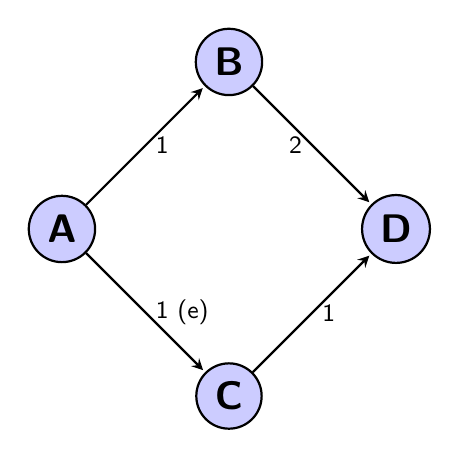
\begin{tikzpicture}[->,>=stealth,shorten >=1pt,auto,node distance=3cm,
 		thick,main node/.style={circle,fill=blue!20,draw,font=\sffamily\Large\bfseries}]

  		\node[main node] (B) {B};
  		\node[main node] (A) [below left of=B] {A};
  		\node[main node] (C) [below right of=A] {C};
  		\node[main node] (D) [below right of=B] {D};

  		\path[every node/.style={font=\sffamily\small}]
    		(B) edge node [left] {2} (D)
    		(A) edge node [right] {1} (B)
        		edge node [right]  {1 (e)} (C)
    		(C) edge node [right] {1} (D);
		\end{tikzpicture}\\
		With edge $e$ as noted (connecting A to C), then $e$ can be part of a min cut.  The max flow of the system is currently 2.  However, if we increase $c(e)$ to 2, then the max flow of the system is still 2, and $e$ is no longer part of a min cut.
	\item Let $z=min(x+y,y+w,3x+w)$.  Then \\
	max $z$\\
	$x + y - z \geq 0 \\
	y + w - z \geq 0\\
	3x + w - z \geq 0\\
	x + y + w = 1$ 
	\item If we relax the integrality constraints, we can turn the integer linear program into a linear program.  Once we find the optimal solution to this linear program, we need to transform it into a valid vertex cover and show that it is a 2-approximation of the optimal.\\
	To turn the optimal solution into a valid vertex cover, we can take all the vales of $x_u$ and round them to the nearest integer (i.e. $x_u \geq 1/2$ becomes $1$, $x_u < 1/2$ becomes $0$).  This will ensure a valid cover: if $x_u+x_v\geq 1$, $\Call{Round}{x_u} + \Call{Round}{x_v} \geq 1$, because at least one of $x_u$ or $x_v$ must be $\geq 1/2$.  Let's call the valid cover $C = {x_u \in V s.t. \Call{round}{x_u} = 1}$\\
	This rounded optimal solution is a 2-approximation of the true optimal solution because its cost is $\sum\limits_{v \in C}^{} c(v) = \sum\limits_{v \in V}^{} c(v) * \Call{Round}{x_v} \leq \sum\limits_{v \in C}^{} c(v) * 2 * \Call{Unrounded}{x_v} = 2*(optimallinearsolution) \leq 2*(optimalvertexcover)$.
	\item A is $C(f(s_I) , t) + v_I$.\\B is $C(t, f(s_I)) + v_I$.
	\item Assuming $f(x)$ is $O(1)$ and using $n$ to represent the number of intervals, the running time of the above dynamic program is $O(n^2)$.
	\end{enumerate}
\item Point domination
	\begin{enumerate}
	\item An efficient ($O(n^2)$) algorithm to find all points of set $S$ which do not dominate any other point in $S$:
		\begin{algorithmic}
		\State $nondominatingpoints \gets []$
		\For{$p_i = (x_i , y_i ) \in S$}
			\State $dominates \gets false$
			\For{$p_j = (x_j, y_j) \in S - p_i$}
				\If{$x_i > x_j $and $y_i > y_j$}
					\State $dominates \gets true$
				\EndIf
			\EndFor
			\If{$dominates$}
				\State continue
			\EndIf
			\State $nondominatingpoints \gets [nondominatingpoints, p_i]$
		\EndFor
		\end{algorithmic}
	\item An efficient algorithm to find the largest subset of points $U \subset S$ where for each pair of points in $U$ neither dominates the other, the basic idea of which is to sort by increasing $x$, then create a DAG in which there are edges connecting from points of higher $y$ to points of lower $y$ (that still respect the sorted order), and then find the longest run of connected nodes, in the same manner as the longest increasing subsequence in a DAG:
		\begin{algorithmic}
		\State \# we sort our points by increasing x using mergesort
		\State \# which implementation we omit here
		\State $P \gets mergesort(S)$
		\State $E \gets \{(p_i, p_j): p_i, p_j \in P, p_i[x] < p_j[x], p_i[y] < p_j[y]\}$
		\For{$j = 1, 2, ..., n:$}
			\State $L(j) = 1 + $max$\{L(i) : (i, j) \in E\}$
		\EndFor
		\State \Return max$_j L(j)$
		\end{algorithmic}
	\end{enumerate}
\item Clauses\\
	 Intuitively, if we have $n$ true colors, we want to connect each clause vertex $v$ to $n$ other clauses which, if they were all satisfiable, would ensure that $v$ was not satisfiable.  For example, we could connect the vertex for clause $(x_i, x_j, \overline{x_k})$ to vertices representing $(x_i, x_j, x_k), (\overline{x_i}, x_j, \overline{x_k}), (x_i, \overline{x_j}, \overline{x_k}), (\overline{x_i}, \overline{x_j}, x_k)$ (or whatever subset thereof is contained in the set of clauses), because if all four of those clauses are satisfiable then $(x_i, x_j, \overline{x_k})$ is not.  In addition to those connections, we also want to connect $(x_i, x_j, \overline{x_k})$ to the example three-variable gadget at the vertices representing each of its component literals, i.e. $v_i, v_j, v_k '$, since the assignment of those variables as true or false also determines whether the clause is satisfiable.
\item Pattern Subsequences
	\begin{enumerate}
	\item An $O(nm)$ algorithm for finding any occurrence of $s_1$ within $s_2$ with $k$ or fewer mismatched bits:
		\begin{algorithmic}
		\State $matchlocations \gets [ ]$
		\State $i \gets 0$
		\For{$i < n$}
			\State $count \gets 0$
			\State $j \gets 0$
			\For{$j < m$}
				\If {$s_2[i+j] != s_1[j]$}
					\State $count++$
				\EndIf
				\State $j \gets j + 1$
			\EndFor
			\If {$count < k$}
				\State $matchlocations \gets (matchlocations, i)$
			\EndIf
			\State $i \gets i + 1$
		\EndFor
		\State return $matchlocations$
		\end{algorithmic}
	\item An $O(n log n)$ algorithm for any $k$; we begin by replacing all $0$s with $-1$s, such that in convolution if two bits are the same their product is $1$, and if they differ their product is $-1$. This algorithm uses the idea that the inner product of a substring of $s_1$ and the string $s_2$ (with these replacements) will be maximized (maximum is $m$) if all bits are the same.  For each bit that is different, it reduces the inner product by $1$.  Therefore if less than $k$ bits are different, then the inner product of the two substrings will be $> m-k$:
		\begin{algorithmic}
		\State replace all $0$ in $s_1$ with $-1$
		\State replace all $0$ in $s_2$ with $-1$
		\State $matchlocations \gets [ ]$
		\For{$idx = 1, 2, ... n-m$}
			\State $innerproduct = \Call{FFT}{s_1 substring [idx:idx+m], s_2 }$
			\If{$innerproduct > m-k$}
				\State $matchlocations \gets [matchlocations, idx]$
			\EndIf
		\EndFor
		\State \Return $matchlocations$
		\end{algorithmic}
	\end{enumerate}
\item Sorting by Reversals
	\begin{enumerate}
	\item An absolute lower bound on the number of reversals required to sort a permutation $\pi$ which has $b(\pi)$ breakpoints is $\lceil \frac{b(\pi)}{2} \rceil$.\\
	First, it is not possible to have a list with only $1$ breakpoint.
	\begin{proof}
	If a list $L =$ [$0, \pi_1, \pi_2, ... \pi_n$] had only one breakpoint, it would imply that $\exists \pi_i \in L$ such that $\lvert \pi_{i-1} - \pi_i \rvert = 1$ or $\lvert \pi_{i+1} - \pi_i \rvert = 1$, and $\forall \pi_j \in L, j \neq i, \pi_j = j$.\\
	WLOG, say $\lvert \pi_{i-1} - \pi_i \rvert = 1$ .  This means that the breakpoint is between $\pi_i$ and $\pi_{i+1}$, so either $\pi_i \neq i$ or $\pi_i+1 \neq i+1$.  We must to reverse some portion of the list to attain the state that $\pi_i = i$.  However, we cannot, because $\forall \pi_j \in L, j \neq i, \pi_j = j$, so $i$ is not present elsewhere in the list.
	\end{proof}
	We can resolve at most $2$ breakpoints with a single reversal.
	\begin{proof}
	If we begin with a list $0, \pi_1, \pi_2, ... , \pi_n, n+1$ and we reverse the list between $\pi_i$ and $\pi_j$, then we do not change the number of breakpoints in the segments [$0, \pi_1, ... \pi_{i-1}$], [$\pi_i, \pi_{i+1}, ... , \pi_j$], or [$\pi_{j+1}, ... \pi_n, n+1$].  Either $\rvert \pi_{i-1} - \pi_j \lvert = 1$ or not and either $\rvert \pi_i - \pi_{j+1} \lvert = 1$ or not.  So our possible breakpoint resolutions are 0, 1, or 2.
	\end{proof}
	In the case where a list has three breakpoints, with any reversal we perform, we can resolve at most one breakpoint, thus reducing the problem to the above.
	\begin{proof}
	If a list $L$ has exactly $3$ breakpoints, is of the form $0, 1, ...,i-1, i, i+2, i+3, ... i+j, i+j+1, i+1, i+j+2, i+j+3, ..., n, n+1$.  In this case, we do not want to perform a reversal on any sublist between $0$ and $i$, since those elements are already in order and doing so would introduce a break point.  For the same reason, we do not want to perform a reversal on any sublist between $i+2$ and $i+j+1$ or between $i+j+2$ and $n+1$.  Therefore, we can reverse the list between $i+2$ and $i+j+1$ or between $i+2$ and $i+1$.\\
	In the first case, we create the list $0, 1, ...,i-1, i, i+j+1, i+j, ... i+3, i+2, i+1, i+j+2, i+j+3, ..., n, n+1$, which has $2$ breakpoints.  In the second case, we create the list $0, 1, ...,i-1, i, i+1, i+j+1, ... i+3, i+2, i+j+2, i+j+3, ..., n, n+1$, which has $2$ breakpoints.  Therefore, we can resolve at most one breakpoint with a single reversal in a list with three breakpoints.
	\end{proof}
	In an ideal situation, if $b(\pi)$ is even we could continue resolving $2$ breakpoints until we have $0$ breakpoints, and if $b(\pi)$ is odd we can resolve $2$ breakpoints per reversal until we have $3$ breakpoints (since we cannot have only $1$ breakpoint).  We can then perform a reversal to resolve $1$ breakpoint, leaving us with $2$, and perform the final reversal.\\
	Therefore, the lower bound of the number of reversals needed to resolve $b(\pi)$ breakpoints is $\lceil \frac{b(\pi)}{2} \rceil$.
	\item
	\begin{algorithmic}
	\Function{nextreverse}{$list$}
		\For{$i = 0, 1, ..., n+1$}
			\If{$list[i] \neq i$}
				\State \#find where it is, and if its neighbours follow
				\State choose $j$ such that $\pi_j = i \in list$
				\While{$j < n$ and $\pi_{j+1} - \pi{j} = 1$}
					\State $j \gets j+1$
				\EndWhile
				\Return $\pi_j$
			\EndIf
		\EndFor
		\Return $n+1$
	\EndFunction\\
	\While{ ($i \gets $\Call{nextreverse}{$permutedlist$}) $\neq n+1$}
		\State choose $j$ such that $\pi_j = i \in permutedlist$
		\State $\rho[\pi_i:j]$
	\EndWhile
	\end{algorithmic}
	This algorithm resolves at least one breakpoint per two reversals: it finds the first $\pi_j = i$ that is not located at index $i$ in the list, then searches beyond it to see whether its proper neighbors follow; that is, what is the largest $k$ such that $\pi_{j+k} = i+k$ is true for $0, ..., k$.  It then performs $\rho(i, j+k)$ to get the long list of neighbors correctly situated in place from index $i$ to index $i+k$.  It then reverses that list, which resolves the breakpoint between $i+1$ and $i$, thereby solving at least one breakpoint in two reversals.  This means that this algorithm is within 4 of optimal, since $1/2$ breakpoint per reversal multiplied by $4$, is $2$ breakpoints per reversal.
	\end{enumerate}
\end{enumerate}
\end{document}